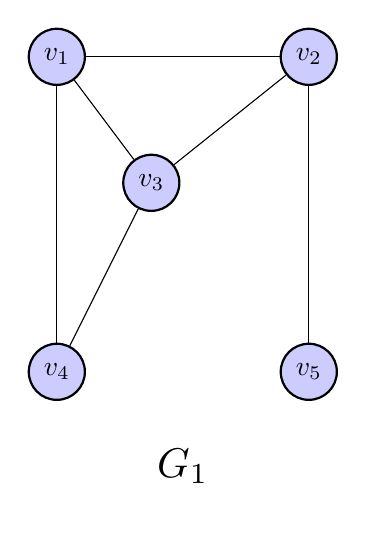
\begin{tikzpicture}[scale=.8,auto=left,every node/.style={circle,fill=blue!20,draw=black,thick}]
  % Vértices G1
  \node (n1) at (0, 4) {$v_1$};
  \node (n2) at (4, 4) {$v_2$};
  \node (n3) at (1.5, 2) {$v_3$};
  \node (n4) at (0, -1) {$v_4$};
  \node (n5) at (4, -1) {$v_5$};

  % Aristas G1 (Quitando n2/n4)
  \foreach \from/\to in {n1/n2, n1/n3, n1/n4, n2/n3, n2/n5, n3/n4}
    \draw (\from) -- (\to);

  % Título
  \node[draw=none, fill=none, scale=1.5] at (2, -2.5) {$G_1$};
\end{tikzpicture}
